\documentclass[journal,12pt,twocolumn]{IEEEtran}
\usepackage{setspace}
\usepackage{gensymb}
\usepackage{tabularx}
\singlespacing
\usepackage{float}
\usepackage{graphicx}
\usepackage{amsmath}
\usepackage{amsthm}
\usepackage{mathrsfs}
\usepackage{txfonts}
\usepackage{stfloats}
\usepackage{bm}
\usepackage{cite}
\usepackage{cases}
\usepackage{subfig}
%\usepackage{xtab}
\usepackage{longtable}
\usepackage{multirow}
%\usepackage{algorithm}
%\usepackage{algpseudocode}
\usepackage{enumitem}
\usepackage{mathtools}
\usepackage{tikz}
\usepackage{circuitikz}
\usepackage{verbatim}
%\usepackage{tfrupee}
\usepackage[breaklinks=true]{hyperref}
%\usepackage{stmaryrd}
\usepackage{tkz-euclide} % loads  TikZ and tkz-base
%\usetkzobj{all}
\usepackage{listings}
    \usepackage{color}                                            %%
    \usepackage{array}                                            %%
    \usepackage{longtable}                                        %%
    \usepackage{calc}                                             %%
    \usepackage{multirow}                                         %%
    \usepackage{hhline}                                           %%
    \usepackage{ifthen}                                           %%
  %optionally (for landscape tables embedded in another document): %%
    \usepackage{lscape}     
\usepackage{multicol}
\usepackage{chngcntr}
\def\inputGnumericTable{}                                
%\usepackage{enumerate}

%\usepackage{wasysym}
%\newcounter{MYtempeqncnt}
\DeclareMathOperator*{\Res}{Res}
%\renewcommand{\baselinestretch}{2}
\renewcommand\thesection{\arabic{section}}
\renewcommand\thesubsection{\thesection.\arabic{subsection}}
\renewcommand\thesubsubsection{\thesubsection.\arabic{subsubsection}}

\renewcommand\thesectiondis{\arabic{section}}
\renewcommand\thesubsectiondis{\thesectiondis.\arabic{subsection}}
\renewcommand\thesubsubsectiondis{\thesubsectiondis.\arabic{subsubsection}}

% correct bad hyphenation here
\hyphenation{op-tical net-works semi-conduc-tor}
\def\inputGnumericTable{}                                 %%

\lstset{
%language=C,
frame=single, 
breaklines=true,
columns=fullflexible
}
%\lstset{
%language=tex,
%frame=single, 
%breaklines=true
%}

\begin{document}
%


\newtheorem{theorem}{Theorem}[section]
\newtheorem{problem}{Problem}
\newtheorem{proposition}{Proposition}[section]
\newtheorem{lemma}{Lemma}[section]
\newtheorem{corollary}[theorem]{Corollary}
\newtheorem{example}{Example}[section]
\newtheorem{definition}[problem]{Definition}
%\newtheorem{thm}{Theorem}[section] 
%\newtheorem{defn}[thm]{Definition}
%\newtheorem{algorithm}{Algorithm}[section]
%\newtheorem{cor}{Corollary}
\newcommand{\BEQA}{\begin{eqnarray}}
\newcommand{\EEQA}{\end{eqnarray}}
\newcommand{\define}{\stackrel{\triangle}{=}}

\bibliographystyle{IEEEtran}
%\bibliographystyle{ieeetr}


\providecommand{\mbf}{\mathbf}
\providecommand{\pr}[1]{\ensuremath{\Pr\left(#1\right)}}
\providecommand{\qfunc}[1]{\ensuremath{Q\left(#1\right)}}
\providecommand{\sbrak}[1]{\ensuremath{{}\left[#1\right]}}
\providecommand{\lsbrak}[1]{\ensuremath{{}\left[#1\right.}}
\providecommand{\rsbrak}[1]{\ensuremath{{}\left.#1\right]}}
\providecommand{\brak}[1]{\ensuremath{\left(#1\right)}}
\providecommand{\lbrak}[1]{\ensuremath{\left(#1\right.}}
\providecommand{\rbrak}[1]{\ensuremath{\left.#1\right)}}
\providecommand{\cbrak}[1]{\ensuremath{\left\{#1\right\}}}
\providecommand{\lcbrak}[1]{\ensuremath{\left\{#1\right.}}
\providecommand{\rcbrak}[1]{\ensuremath{\left.#1\right\}}}
\theoremstyle{remark}
\newtheorem{rem}{Remark}
\newcommand{\sgn}{\mathop{\mathrm{sgn}}}
\providecommand{\abs}[1]{\left\vert#1\right\vert}
\providecommand{\res}[1]{\Res\displaylimits_{#1}} 
\providecommand{\norm}[1]{\left\lVert#1\right\rVert}
%\providecommand{\norm}[1]{\lVert#1\rVert}
\providecommand{\mtx}[1]{\mathbf{#1}}
\providecommand{\mean}[1]{E\left[ #1 \right]}
\providecommand{\fourier}{\overset{\mathcal{F}}{ \rightleftharpoons}}
%\providecommand{\hilbert}{\overset{\mathcal{H}}{ \rightleftharpoons}}
\providecommand{\system}{\overset{\mathcal{H}}{ \longleftrightarrow}}
	%\newcommand{\solution}[2]{\textbf{Solution:}{#1}}
\newcommand{\solution}{\noindent \textbf{Solution: }}
\newcommand{\cosec}{\,\text{cosec}\,}
\providecommand{\dec}[2]{\ensuremath{\overset{#1}{\underset{#2}{\gtrless}}}}
\newcommand{\myvec}[1]{\ensuremath{\begin{pmatrix}#1\end{pmatrix}}}
\newcommand{\mydet}[1]{\ensuremath{\begin{vmatrix}#1\end{vmatrix}}}
%\numberwithin{equation}{section}
%\numberwithin{equation}{subsection}
%\numberwithin{problem}{section}
%\numberwithin{definition}{section}
\makeatletter
\@addtoreset{figure}{problem}
\makeatother

\let\StandardTheFigure\thefigure
\let\vec\mathbf
%\renewcommand{\thefigure}{\theproblem.\arabic{figure}}
\renewcommand{\thefigure}{\theproblem}
%\setlist[enumerate,1]{before=\renewcommand\theequation{\theenumi.\arabic{equation}}
%\counterwithin{equation}{enumi}


%\renewcommand{\theequation}{\arabic{subsection}.\arabic{equation}}

\def\putbox#1#2#3{\makebox[0in][l]{\makebox[#1][l]{}\raisebox{\baselineskip}[0in][0in]{\raisebox{#2}[0in][0in]{#3}}}}
     \def\rightbox#1{\makebox[0in][r]{#1}}
     \def\centbox#1{\makebox[0in]{#1}}
     \def\topbox#1{\raisebox{-\baselineskip}[0in][0in]{#1}}
     \def\midbox#1{\raisebox{-0.5\baselineskip}[0in][0in]{#1}}

\title{FWC IDE ASSIGNMENT\\ \normalsize Parv Chandola}
\maketitle
%\tableofcontents


Q.The circuit shown in the figure below uses ideal positive edge-triggered synchronous J-K flip flops with outputs X and Y. If the initial state of the output is X=0 and Y=0, just before the arrival of the first clock pulse, the state of the output just before the arrival of the second clock pulse is

\begin{figure}[!h]
	\begin{center} 
	    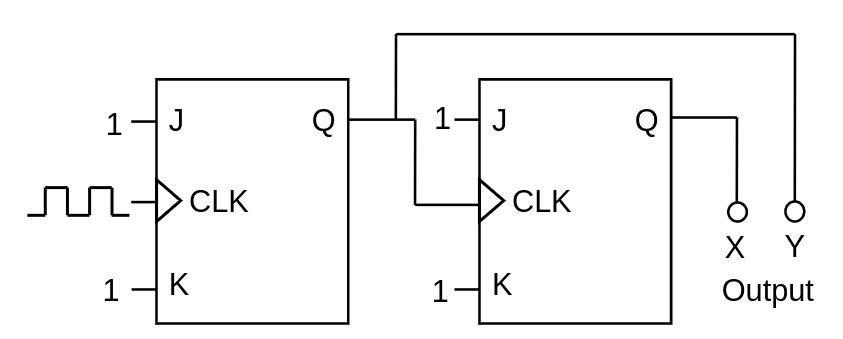
\includegraphics[width=\columnwidth]{figs/cir}
	\end{center}
\caption{}
\label{fig:Fig1}
\end{figure}

\solution

The output equation for a J-K flip flop is given as:
\begin{align}
Q_{n+1} = J\bar{Q_{n}} + \bar{K}Q_{n}
\end{align}

So if J=1 and K=1 then
\begin{align}
Q_{n+1} = \bar{Q_{n}}
\end{align}

Since the 2nd J-K flip flop clock input comes from the output of the first flip flop so 2nd J-K flip flop will be triggered when output of 1st flip flop goes from low to high(as the flip flops are positive edge triggered).

The Table \ref{table:1} below shows the output states of the flip flops.

\begin{table}[h!]
\begin{center}
\begin{tabular}{ | m{2em} |m{0.5cm}|m{0.5cm}| m{0.8cm}| m{0.8cm} |m{1.5cm} |m{1.5cm} | } 
  \hline
  \textbf{Clock}& J &K &{$Q_{0}(n)$} & {$Q_{1}(n)$}&{$Q_{0}(n+1)$}&{$Q_{1}(n+1)$} \\ 
  \hline
  1 &1 &1 & 0 & 0& 1& 1 \\ 
  \hline
  2 & 1 &1 &1 & 1& 1& 0 \\ 
  \hline
  3 &1 &1 & 1 & 0 & 0& 1\\
  \hline
  4& 1 &1 &0 & 1 & 0& 0\\
  \hline
  5&1 &1 & 0 & 0 & 1& 1\\
  \hline
\end{tabular}
\caption{}
\label{table:1}
\end{center}
\end{table}

From the different states we get to know that the next state of the flip-flop after the first clock pulse is 
\textbf{X=1},\textbf{Y=1}. And the above circuit is behaving like a decreament counter.


Given below are the codes of IDE, Assembly and AVR-gcc respectively for the above problem implementation.

\begin{lstlisting}
https://github.com/ParvChandola/FWC1/blob/main/assignments/ide/IDE.ino
\end{lstlisting}

\begin{lstlisting}
https://github.com/ParvChandola/FWC1/blob/main/assignments/ide/assembly.asm
\end{lstlisting}

\begin{lstlisting}
https://github.com/ParvChandola/FWC1/blob/main/assignments/ide/AVRgcc.c
\end{lstlisting}
The connection are given in the Table \ref{table:2}.

\newpage
\begin{table}[h!]
\begin{center}
\begin{tabular}{ | m{5em} | m{1cm}| m{1cm} |m{1cm} |m{1cm} |m{2.5cm} |m{3cm} |m{2cm} | } 
  \hline
  \textbf{Arduino} & 2 & 3& 6& 7& 13& 5V& GND \\ 
  \hline
  \textbf{7474} & 2 & 12 & 5&9 & CLK1,CLK2& 1,4,10,13,14& 7\\ 
  \hline
  \textbf{7447} & 7 & 1 & & & & 16& 2,6,8\\ 
  \hline
\end{tabular}
\caption{}
\label{table:2}
\end{center}
\end{table}

\end{document}


